% !TEX root = ../../fyp.tex
\documentclass[../../fyp.tex]{subfiles}

\begin{document}
\subsection{What are the fundamentals of a Neural Network?}
Modelled on the human brain, neural networks typically involve a series of layers composed of neurons. Figure \ref{fig:ffnn} illustrates one such simplified neural network architecture with a single hidden layer, $L_2$, preceded by the input layer $L_1$, and followed by the output layer $L_3$. $(x_1, x_2, x_3)$ represents a three dimensional input vector, whereas the neurons, or hidden units, of the of the network are depicted as $(h_1, h_2, h_3)$. The firing action of each neuron is expressed using a non-linear activation function. This action propagates from one neuron in a layer to all other connected neurons in the subsequent layer and is modulated by a particular weight that characterizes each intra-neural connection. At minimum, these networks will incorporate an input and an output layer that will encapsulate one, or more, hidden layers.

The network is able to learn, or model, a function by adjusting the weights to minimize a some measure of error towards a particular objective function. \cite{graves2012b}

The hidden layers of a neural network architecture are able to extrapolate features at a level that cannot be carried out manually, thereby capturing more subtle details and generating richer representations of the data being learned. Foregoing this need for extensive manual feature engineering is one of the primary drivers of neural network models, even though these are approaches are typically black-box solutions, with obfuscated inner-workings.

\begin{figure}[!ht]
	\centering
	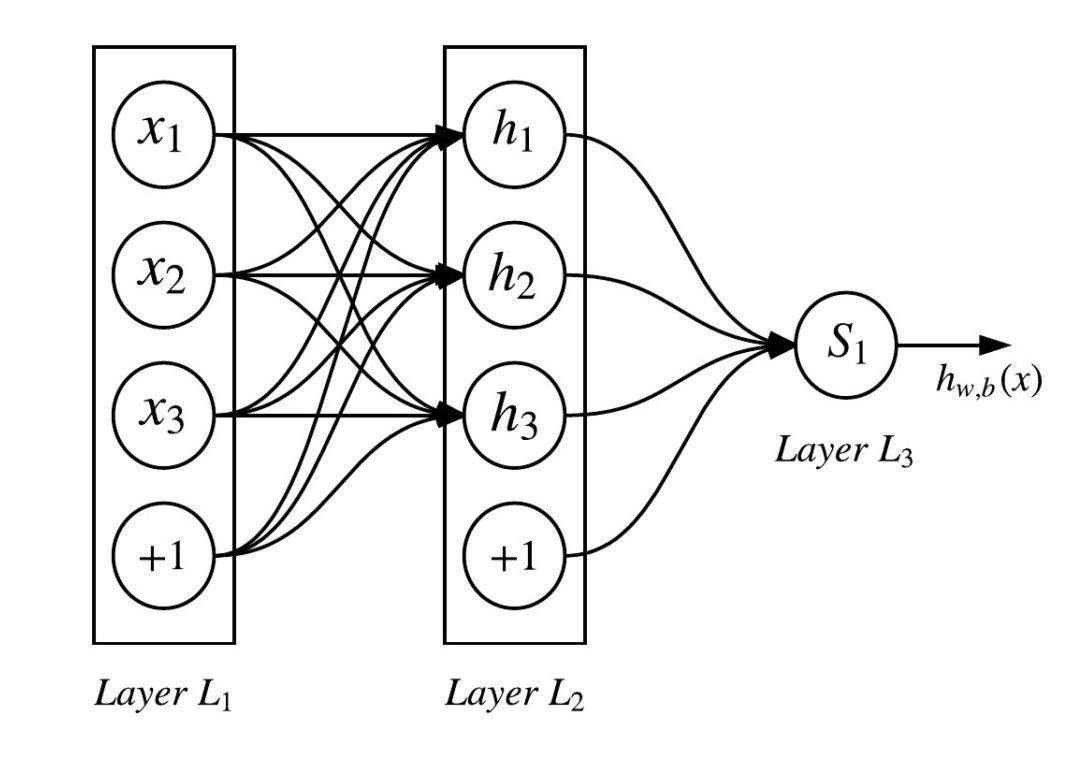
\includegraphics[width=0.7\textwidth]{ffnn.jpg}
	\caption{Standard feedforward neural network (FFNN) architecture \cite{zhang2018}}
	\label{fig:ffnn}
\end{figure}

\subsection{What are the common activation functions?}
Three of the most commonly used activation functions are sigmoid (eq. \ref{eq:sigmoid}), hyperbolic tangent (eq. \ref{eq:hyperbolic_tangent}) and Rectified Linear Unit (ReLU; eq. \ref{eq:relu}). Although the choice of activation function is typically heuristic, \cite{glorot2011} as cited in \cite{zhang2018} notes that the ReLU is easier to compute when compared to the other two and also tends to converge faster, all while maintaining similar or even better performance.

\begin{equation} \label{eq:sigmoid}
	f(W^tx) = sigmoid(W^tx) = \frac{1}{1+e^{-W^tx}}
\end{equation}
\begin{equation} \label{eq:hyperbolic_tangent}
	f(W^tx) = \tanh(W^tx) = \frac{e^{W^tx}-e^{-W^tx}}{e^{W^tx}+e^{-W^tx}}
\end{equation}
\begin{equation} \label{eq:relu}
	f(W^tx) = ReLU(W^tx) = \max(0,W^tx)
\end{equation}

\subsection{How are Neural Networks typically trained?}
Neural networks are trained by following the direction of the gradient that lessens the measured error rate of some objective function which is calculated through the repeated application of the chain-rule. The process can be carried out on the training set in its entirety, commonly referred to as batch learning, or in an on-line manner, carrying out updates after each training sample. The latter is known as stochastic gradient descent and is known to be more efficient and robust to local minima when dealing with large datasets \cite{lecun1998} as cited in \cite{graves2012b}.

There will always be noise in the sampled training data that does not translate to the real world test data scenarios and that the model must therefore avoid learning. Training models to the point of becoming overly-sensitive to this noise is referred to as over-fitting the data, and there are a number of regularization techniques often employed in the literature while training to counteract this.

One common approach is introducing some form of weight penalties, for instance, $L1$ and $L2$ regularization. Other techniques frequently used include \textit{early-stopping}, whereby a fraction of the training data is used as a validation set that the model is tested against at regular intervals during training to test for a sustained improvement \cite{graves2012}, and \textit{dropout} \cite{srivastava2014}, in which random neurons in a NN are ignored (\enquote{dropped}) with some probability $p$, effectively training a diverse range of \enquote{thinned} versions of the original NN. An approximated average of those networks is subsequently used as final trained model by scaling its weights by that same dropout probability $p$.

\subsection{How are Deep Neural Networks formed?}
\enquote{Deep} neural networks are constructed by stacking a series of layers in such a way that salient features extracted from one layer are passed on as input data to the next layer, and so on. This stacking process, in theory, improves the capacity of the network to extract more abstract and expressive features that reside at a deeper level within the input data. \cite{zhang2018}

\subsection{Why is Deep Learning popular again recently?}
In recent years, the astounding progress in computing resources such as GPUs and high performance distributed computing have made deep learning accessible on an unparalleled level. Consequently, this has driven interest in the applicability of deep learning architectures such as the CNN and RNN in a range of fields from computer vision to natural language processing \cite{goldberg2015}, \cite{collobert2011}.

\subsection{What are two common deep learning models used? (CNN and RNN)}
Not least owing to their impeccable ability for effectively extracting highly expressive low-dimensional representations of text automatically, coupled with the aforementioned resurgence of deep learning due to the increase in available computing power, the use of neural network models such as \cite{lakkaraju2014} \cite{vo2015} \cite{nguyen2015}  became increasingly widespread within the field of NLP, including targeted and aspect based sentiment classification tasks \cite{dong}; \cite{wang}; \cite{tang2016} \cite{tang2016b}.

The most prevalent architectures are the Convolutional Neural Networks (CNNs) and Recurrent Neural Networks (RNN) and the descendents thereof. Other deep learning models worth mentioning include the Recursive Neural Network (Rec-NN), which has been employed in works such as \cite{socher2011} and \cite{socher2013} for syntactic analysis and sentence sentiment analysis respectively. \cite{zhang2018}

\subsection{What are the fundamentals of a CNN (in brief)?}
The layers typically comprise of filters, also referred to as kernels, of differing widths that slide over the input data to extrapolate various features. Each of these features would be representative of a diverse set of aspects of the data that would aid in defining it with respect to the task being tackled.

These convolution layers are coupled with a max-pooling layer with the intention of extracting the most salient values. These values can subsequently be forwarded to another convolution layer that presumably extrapolates deeper, more abstract features. This process can be repeated a number of times across multiple convolution layers to build a deep CNN that eventually produces a single feature vector representation of the original input data. Figure \ref{fig:cnn_architecture} illustrates this process using six filters with three difference widths and two diverse operations for each, the results of which are down-scaled using max-pooling, and subsequently passed through a softmax function for binary classification.

\begin{figure}[!ht]
	\centering
	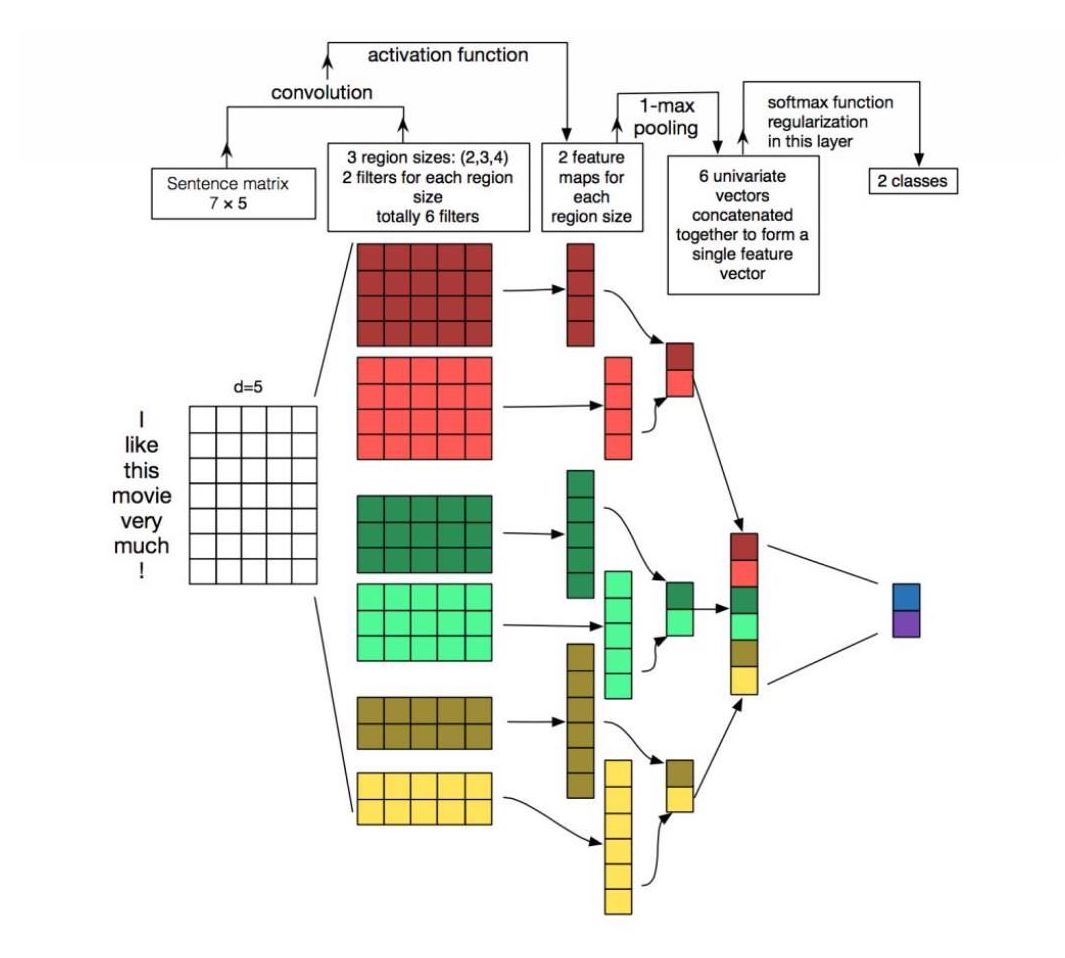
\includegraphics[width=0.7\textwidth]{cnn_architecture.jpg}
	\caption{An example of a CNN architecture used for sentence modelling and subsequent binary classification \cite{yezhang2015} as cited in \cite{young2017}.}
	\label{fig:cnn_architecture}
\end{figure}

\subsection{What are the advantages of using max-pooling?}
Max-pooling is ideal for producing a fixed-length representation of the data, which is a common prerequisite for classification tasks, while at the same time preserving the most prominent features from the original data. \cite{young2017}

\subsection{What are some approaches using CNN?}
Some of the first CNN-based approaches that paved the way for the growth of CNN architectures in the literature that followed were \cite{collobert2011}, \cite{kim}, and \cite{kalchbrenner2014}.
\cite{kim} used CNN architecture for sentence classification tasks ranging from subjectivity and question type with promising results albeit in the face of a number of challenges that became evident to the authors. Not least of these was the limited capacity for the CNN architecture to capture syntactical dependencies in sentences that occurred over long distances. This challenge was the one of the foremost drivers for the work that followed by \cite{kalchbrenner2014} who developed the DynamicCNN (DCNN) which consisted of a series of hierarchical convolution and k-max pooling layers.

Other works cited in \cite{young2017} include \cite{poria2016} that dealt with sarcasm detection on twitter data, noting a need for additional context information when dealing with short texts of this nature. This observation is also echoed in \cite{johnsonzhang2015}, who noted superior performance of CNN networks when dealing with longer text that would provide more contextual information as opposed to shorter text. Due to the vast amount of parameters that CNNs typically need to learn, scarcity of data is an often cited challenge \cite{young2017}.

Work carried out by \cite{chen2016} made use of a CNN to deduce the sentiment of the target based on the sentiment of the clause surrounding it. As noted by \cite{chen2017} however, this method still operated on the assumption that the most salient features of a word can be extracted from other words in close proximity.

A phrase such as \enquote{I bought a mobile phone, its camera is wonderful but the battery life is short, not particularly satisfied overall}, challenges this assumption with respect to the \enquote{mobile phone}, as the intended target since the most sentimentally-laden words appear at the opposite end of the sentence.

\subsection{What are the fundamentals of an RNN based model (in brief)?}
A Recurrent Neural Network (RNN) can be thought of as a chain of recurring modules which typically represent elements within a variable-length sequence, with an internal hidden state that represents the network's \enquote{memory}. This state is passed forward from one module in the chain to the next.

Unlike a CNN, where each layer has its own set of trainable parameters that must be learned, a RNN uses a single set of parameters across all of the modules in the chain which significantly diminishes the total number of parameters that it must learn.

Through forwarding the hidden state from one time step in the chain to the next, the network is able to \enquote{remember} information from previous elements of the sequence and use that information when generating a representation for the current element \cite{tang2016b}.

\subsection{What makes the RNN more suitable for targeted sentiment analysis? (sequence)}
The hidden state that characterizes RNNs acts as its \enquote{memory} element and makes these networks particularly effective in dealing with data that are sequential in nature. One of the most prominent examples of these data is language, where the significance of a word at one time step may be substantially altered by those that preceded it. Consider, for example, the word \enquote{dog}, for which the meaning would shift entirely, from an animal to a popular American snack, should it be preceded by the word \enquote{hot} \cite{young2017}.

Moreover, the capacity of RNNs to model variable length sequences to a fixed length representation also makes them particularly practical when dealing with different units of resolution in languages including documents, sentences, and even words, all of which are naturally arbitrary in length. \cite{tang}

\subsection{What is problem faced by RNN? (vanishing \& exploding gradient)}
In the setting of a traditional RNN, the tendency for a gradient to exhibit exponential change to the degree that prevents substantive learning increases with the length of a sequence \cite{bengio1994} \cite{hochreiter1997}. This phenomenon is what is implied by the terms \enquote{vanishing} or \enquote{exploding} gradients, where the changes observed over time steps often vanish with time or, although less frequently, but with equally devastating results, grow exponentially; hindering the network's capacity for learning.

\subsection{What solutions exist to  vanishing/exploding gradient problem? (LSTM and GRU)}
One class of solutions to the vanishing or exploding gradient problem is to carry out particular modifications on top of the standard stochastic gradient descent algorithm, such as gradient clipping, whereby the norm of the gradient vector is \textit{clipped}, or using second order derivatives, which may or may not be influences to a lesser degree. \cite{chung2014}
The second, and more popular, class of solutions look instead to introduce further sophisticated, additive, non-linearities to the traditional RNN unit. These would selectively carry forward salient features and filter out irrelevant information from previous time steps, as opposed to overwriting the memory content at each time step.

Variants on the standard RNN network were proposed to address the vanishing and exploding gradient issue. The most popular of these being the Long Short Term Memory (LSTM) and, more recently, Gated Recurrent Unit (GRU). Other approaches include, but are not limited to, Residual Networks (Res-Net).

\subsection{What are the fundamentals of the LSTM (in brief)?}
LSTM \cite{hochreiter1997} is an extension on the RNN model that addresses the issue of a vanishing or exploding gradients through the use of gates that control the flow of information from the past states to present states.

To do this, the LSTM introduces three adaptive gates that can be considered additional neural layers on top of the single neural layer that characterizes the typical RNN. The layers introduce an increased level of sophistication in the \enquote{remembering} process from one sequence point to the next.

These gates are commonly referred to as the input, forget and output gate. Moreover the LSTM also maintains a two inner states as opposed to one, namely the cell state and the hidden state.

\begin{figure}[!ht]
	\centering
	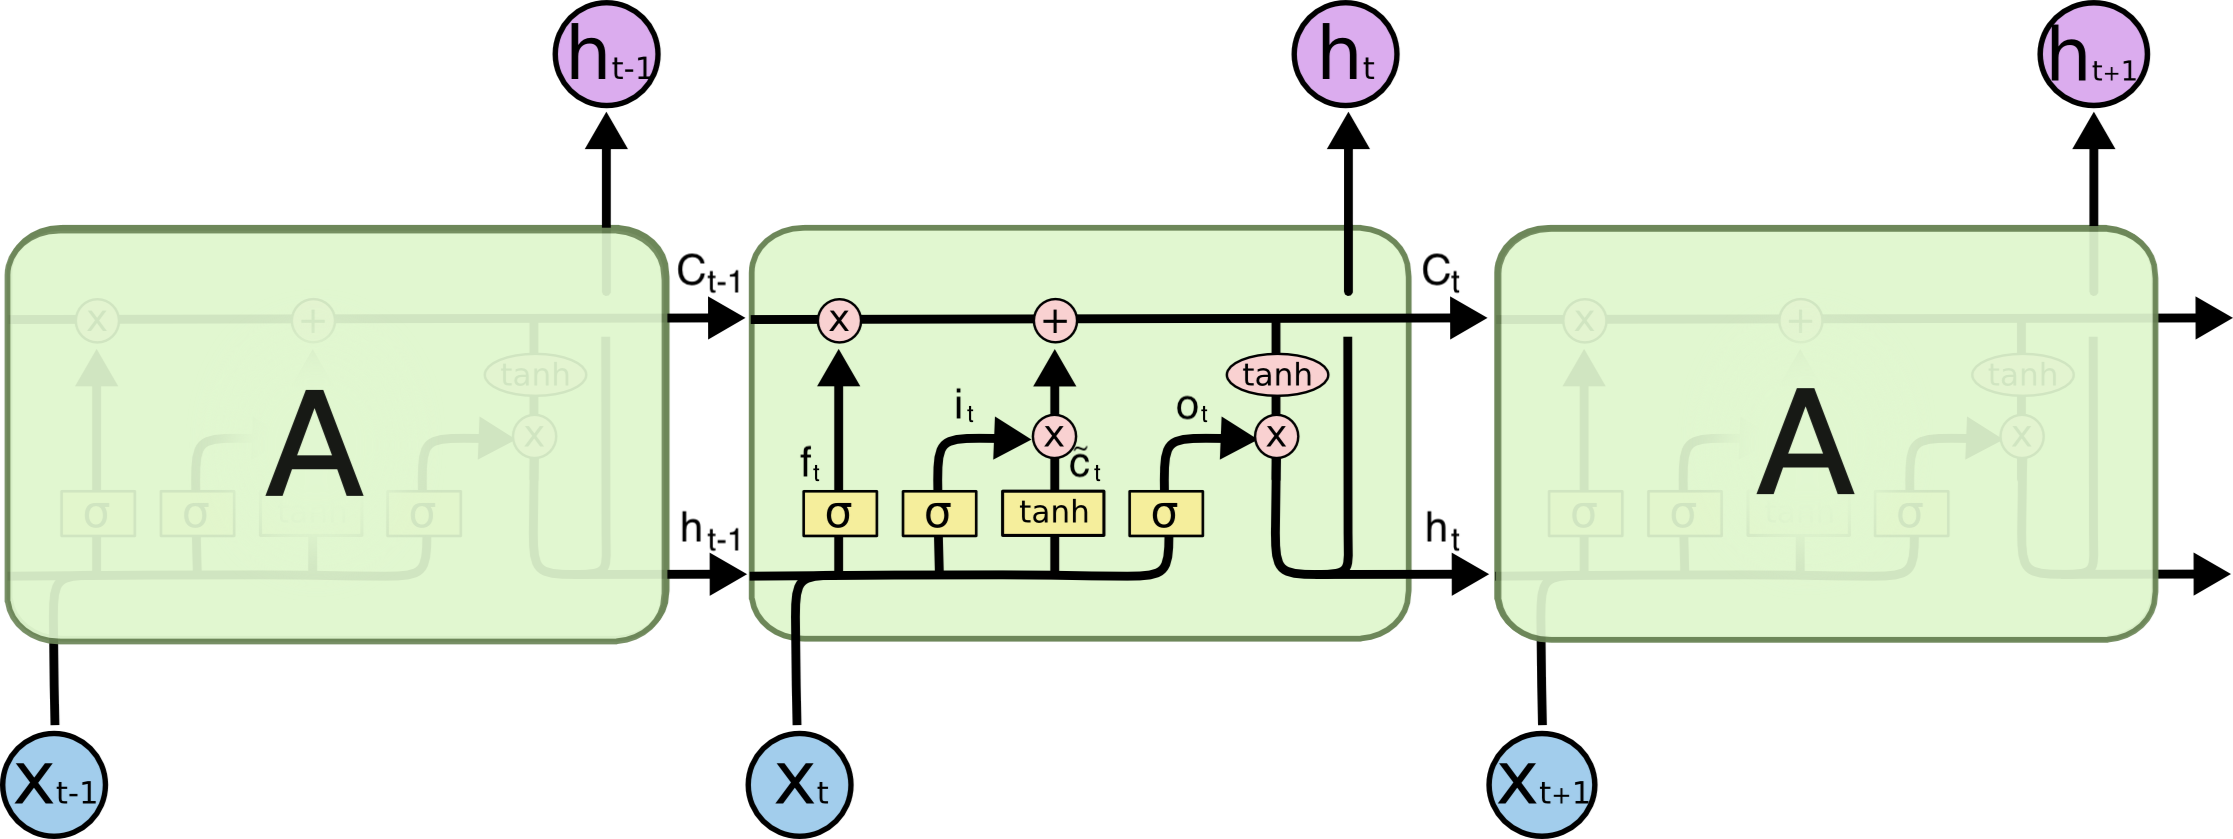
\includegraphics[width=1\textwidth]{lstm_architecture.png}
	\caption{LSTM repeating module illustrating the four neural layers (Yellow Boxes) that comprise it. Point-wise vector operations are depicted in red boxes. Image adapted from \cite{colah-understanding-lstm}}
	\label{fig:lstm_architecture}
\end{figure}

The process undergone in each repeating module of the standard LSTM architecture depicted in figure \ref{fig:lstm_architecture} starts at the forget gate. Here, the information to be removed from the cell state $C_{t-1}$ is selected through the sigmoid layer (eq. \ref{eq:lstm_forget_gate}).
\begin{equation} \label{eq:lstm_forget_gate}
	f_t = \sigma(W_f\cdot[h_{t-1},x_t] + b_f)
\end{equation}
Next, an update vector is produced through a point-wise multiplication operation between the input gate (\ref{eq:lstm_input_gate}), which represents the values selected to be updated, and a vector of candidate values, $\Tilde{C}$ (\ref{eq:lstm_candidate_cell}). This update vector is added to the current cell state, from which the forget gate had previously removed information deemed redundant.
\begin{equation} \label{eq:lstm_input_gate}
	i_t = \sigma(W_i\cdot[h_{t-1},x_t] + b_i)
\end{equation}
\begin{equation} \label{eq:lstm_candidate_cell}
	\Tilde{C} = \tanh(W_C\cdot[h_{t-1},x_t] + b_C)
\end{equation}
Finally, an output gate (\ref{eq:lstm_output_gate}) regulates the amount of cell state information that is output to the rest of the network through the unit's hidden state $h_t$ (eq. \ref{eq:lstm_hidden_state}).
\begin{equation} \label{eq:lstm_output_gate}
	o_t = \sigma(W_o\cdot[h_{t-1},x_t] + b_o)
\end{equation}
\begin{equation} \label{eq:lstm_hidden_state}
	h_t = o_t*\tanh(C_t)
\end{equation}

\subsection{How does the LSTM model address the  vanishing \& exploding gradient problem?}
The gating mechanism that is present in the LSTM network allows for the persistence of salient features that are encountered early in the sequence and which would otherwise be overwritten in a typical RNN architecture.

The input and output gates of the LSTM control the amount of memory content that is to be added to the memory cell and the memory content that is exposed to the rest of the network respectively.

Forget gates were later added to the architecture \cite{gers2000}, which enabled the memory cells to reset themselves. It is important to note that the LSTM updates the memory cell independently from the forget gate, which is to say that, for the LSTM to \enquote{remember} a prior input in a sequence two conditions must be satisfied; the input gate must be closed, preventing the addition of new information and, the forget gate must be maintained open, as otherwise this would cause the existing memory content to be reset.

\subsection{What are some approaches using LSTM?}
\cite{wang} achieved results competitive with those obtained by \cite{kalchbrenner2014} by using an LSTM, as opposed to CNN, to generate representations of tweets. \cite{young2017} notes that their model was able to extract features over long distances at a fraction of the complexity of the DynamicCNN \cite{kalchbrenner2014}.

Another variant on the LSTM architecture involved the use of dependency parsing to build tree-structured LSTMs which operate on some specific tree-pattern that is extracted from the data, typically through the use of external parsing tools \cite{socher2013}. Approaches of this variety \cite{jiweili2015}, \cite{kaishengtai2015}, \cite{zhu2015} have obtained promising results, however as \cite{chen2017} note, these are contingent on the data being well-formed structurally and grammatically, which is not guaranteed when dealing with micro-texts on social media platforms.

Two of the foremost extensions on the classical LSTM model when tackling target-based sentiment analysis, were proposed in \cite{tang2016b} with the intent of accounting for the target information, these were termed the Target Dependent LSTM (TD-LSTM) and Target Connection LSTM (TC-LSTM). Their work showed that the changes proposed would improve the performance over a standard LSTM. \cite{tang2016b} generate representations of a target's left and right contexts, where the target representation is concatenated to each. These two are then finally chained together to form the final, target-specific, representation of the sentence which is fed to an LSTM for sentiment classification \cite{dehongma2017}.

TC-LSTM \cite{tang2016b} was reported as one of the first neural network based methods to obtain state-of-the-art performance without the use of laborious feature engineering and external data sources. It is worth noting however that recent work \cite{moore2018} failed to reproduce the original results that were reported.

\subsection{What are difficulties mentioned that LSTMs deal with?}
While the issue of long-distance dependencies and CNN based approaches is often brought up, \cite{chen2017} remarks that LSTMs will still struggle with features that are located too far apart within a sequence, given the phrase \enquote{Except Patrick, all other actors don’t play well}, an LSTM would struggle to identify the positive sentiment on the opinion target \enquote{Patrick} due to the distance between the terms \enquote{Except} and \enquote{don't play well}.

From the observation made by \cite{bahdanau2014} when employing LSTM-based models in the field of machine translation, \cite{chen2017} make the case that the TD-LSTM would suffer from in instances where the most sentimentally salient word is located further away from the target being considered.

\subsection{How does a Bi-LSTM differ from an LSTM?}
When dealing with bounded sequences, a natural conclusion one  might draw is that valuable information can be extrapolated from future contexts as well as past contexts. Bidirectional RNNs are employed with this specific intention in mind.

Building on top of the LSTM architecture, a Bi-LSTM is so called as it is the result of two stacked LSTMs, each responsible for processing and extracting features from a sequence in opposite directions. Features extracted from these two directions are then typically concatenated into a single, theoretically richer, and more expressive, representation of the sequential data.

It has been argued that the bidirectional nature of these models violates causality, which is justified to an extent, since a future context cannot be exploited if it is the same element that is being predicted. An example of this is predicting future stock market fluctuations. However, for tasks where this information is available, bidirectional variants that make use of this information have consistently been shown to outperform their uni-directional counterparts. \cite{graves2012b}

\subsection{What are some approaches using Bi-LSTM?}
Sentence and document level sentiment classification tasks lend themselves well to the use of bi-directional RNN (BRNN) variants, since the boundaries of the sequence being classified are well-defined a priori. In their work, \cite{chen2017} suggest that using a BLSTM improves the ability of their approach to extrapolate phrase-like features when compared to a uni-directional sequential approach.

An improvement in results stemming, in part, from taking a bi-directional approach is also observed in \cite{zhang2016}, in both accuracy and macro F1 scores when compared to the work of \cite{vo2015}, from which the former was inspired. More recent works (eg. \cite{ma2018}, \cite{zheng2018}) that have reported notable results in the field also take advantage of bi-directionality in their approach.

\subsection{What are the fundamentals of the GRU (in brief)?}
The GRU does away with the cell state that is found in the LSTM, maintaining only a single hidden state as its \enquote{memory}. The second way in which the GRU differs from the LSTM is in its number of gating units, by foregoing the output gate and combining the input and forget gates into a single update gate, the GRU benefits from having less parameters to learn.
\begin{equation} \label{eq:gru_update_gate}
	z_t = \sigma(W_z\cdot[h_{t-1},x_t] + b_z)
\end{equation}
As the name implies, when the reset gate (eq. \ref{eq:gru_reset_gate}) nears $0$, it allows the GRU unit to drop the previous information, which may be deemed inconsequential at a later time, and reset itself with the current input only. This information is then used by the GRU to produce a vector of candidate activation values (eq. \ref{eq:gru_candidate_activation}).
\begin{equation} \label{eq:gru_reset_gate}
	r_t = \sigma(W_r\cdot[h_{t-1},x_t] + b_r)
\end{equation}
\begin{equation} \label{eq:gru_candidate_activation}
	\Tilde{h}_t = \tanh(W\cdot[r_t * h_{t-1},x_t] + b)
\end{equation}

Instead of maintaining an internal memory cell, the GRU uses the update gate and carries out a linear interpolation function (eq. \ref{eq:gru_update_interpolation}) to control the amount of candidate activation, $\Tilde{h}_t$, that is added to the previous activation. In this way the update gate serves as the primary mechanism preventing the GRU from overwriting a previously encountered salient feature.
\begin{equation} \label{eq:gru_update_interpolation}
	h_t = (1-z_t)*h_{t-1} + z_t*\Tilde{h}_t
\end{equation}
Whereas the LSTM utilizes the output gate to control the exposure of its internal memory to the rest of the network, the GRU does not have any means by which to control the exposure of its inner state, and therefore exposes its hidden state in its entirety to the rest of the network.

Each unit in a GRU model will have separate update and reset gates that will independently learn to capture long and short term dependencies in a sequence. Units that learn to capture longer-term dependencies will have active update gates whereas, for short-term dependencies, the reset gates will tend to be more active.

\begin{figure}[!ht]
	\centering
	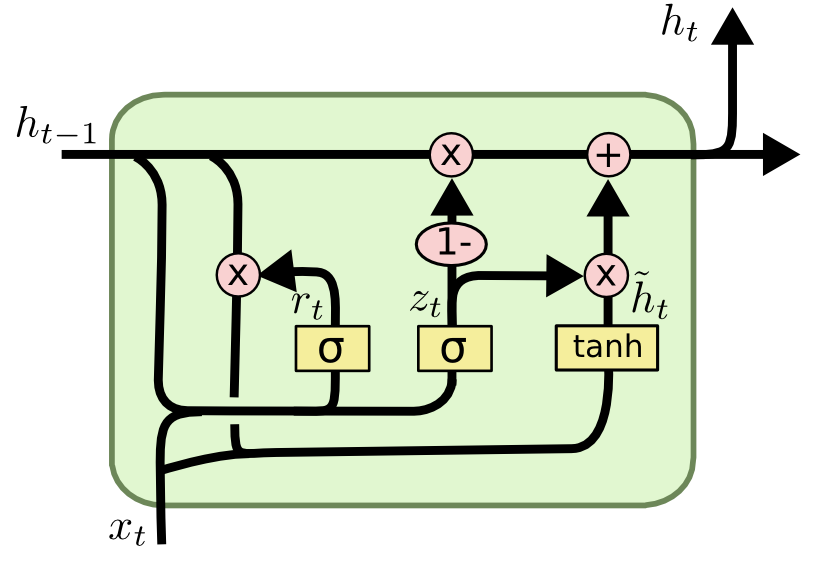
\includegraphics[width=0.7\textwidth]{gru_architecture.png}
	\caption{Internal gating structure of a GRU unit. \cite{colah-understanding-lstm}}
	\label{fig:gru_architecture}
\end{figure}

\subsection{What are some approaches using GRU?}
\cite{zhang2016} model the interplay between targets and their contexts through gated mechanism operating on the a representation of the original sentence split into three components using a gated-RNN.

\cite{liu2018} use a GRU as part of their approach, serving as a gating mechanism to determine whether to update a specific part of memory based on past activations. They claim state of the art results in aspect detection and sentiment classification, outperforming SenticNet \cite{ma2018}, and foregoing the need of external knowledge.

\cite{xue2018} use gated tanh-ReLU units to control flow of features from convolutional neural networks to max pooling layer. They deal more with the advantages that a CNN offers, since it is not time-dependent and is therefore easier to parallelize.

\cite{jabreel2017} generate a sentence representation by stacking two GRU based networks, similar to the BLSTM configuration, opting to go with the GRU architecture instead since it has less parameters to learn, noting similar results. A continuous vector representation of the target is sandwiched between the two GRU direction outputs, and fed to softmax classifier. Authors report accuracy and macro-f1 scores better than state of the art obtained on a twitter dataset \cite{dong}.

\subsection{What advantages/disadvantages does the GRU have over the LSTM if any?}
Since the architecture of the GRU is less complex than that of the LSTM, there may be circumstances where the former may be more efficient than the latter since it requires less parameters to learn \cite{chen2017}, \cite{jabreel2017}.

That being said, there is no clear winner between the two variants, as demonstrated by work conducted in \cite{chung2014}. The results obtained, shown in figure \ref{fig:rnn_v_lstm_v_gru_graphs}, concluded that the only demonstrable advantage is that of both variants over a standard RNN architecture. The authors go on to say that the performance of the two variants themselves is contingent on the particular nature of the tasks being addressed. Although it is worth noting that the work carried out by \cite{chung2014} was not specifically in the field of NLP, the deciding factor between these variants in NLP literature still tends to be heuristic \cite{young2017}.

\begin{figure}[!ht]
	\centering
	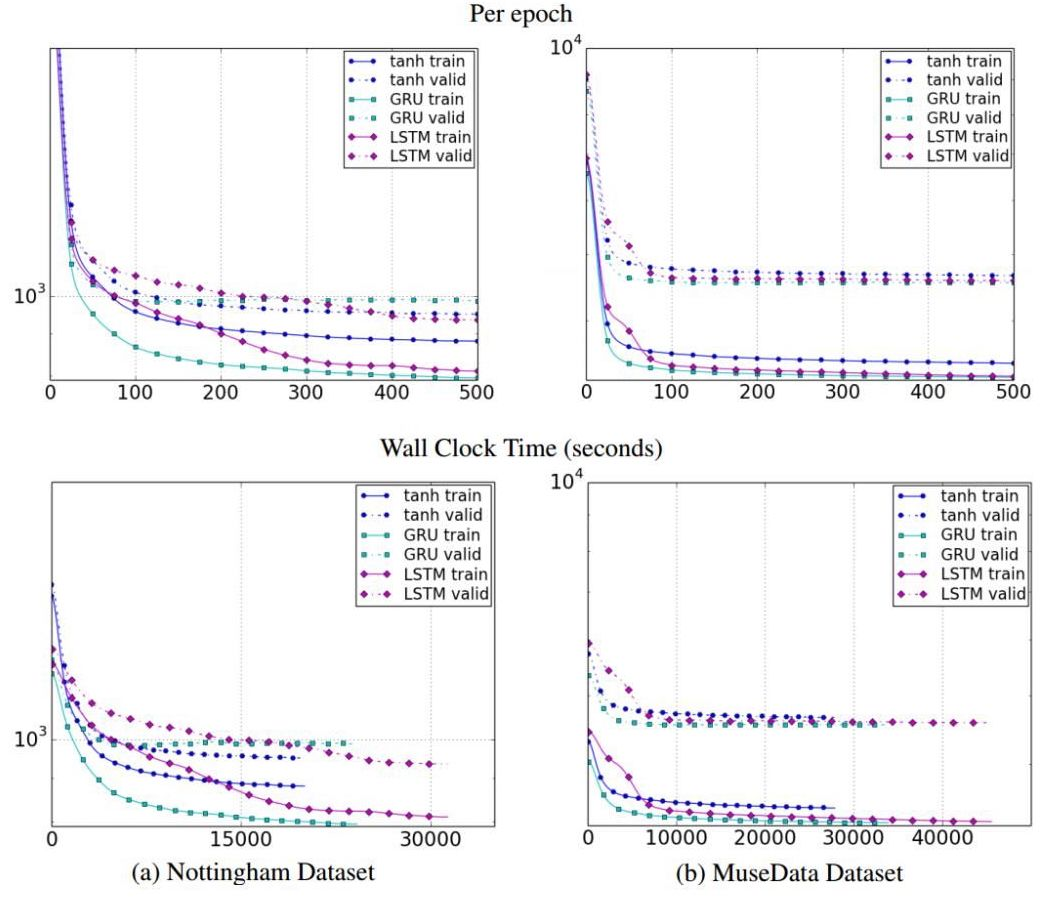
\includegraphics[width=0.7\textwidth]{rnn_v_lstm_v_gru_graphs.jpg}
	\caption{Results obtained by \cite{chung2014} during training and validation of different RNN variants illustrating the superiority of LSTM and GRU units over the traditional RNN.}
	\label{fig:rnn_v_lstm_v_gru_graphs}
\end{figure}

\subsection{Are there any advantages of CNN over RNN models?}
In spite of various studies illustrating the fact that CNN networks are data heavy in nature and often require auxiliary data when dealing with micro-texts such as those obtained from social media networks such as twitter, \cite{young2017} note that assuming the superiority of RNNs for sequential data is inaccurate.

They proceed to cite studies where CNNs performed competitively, and even surpassed RNN-based architectures in tasks for which the latter would, in theory, be better suited, such as language-modelling \cite{dauphin2017} as cited in \cite{young2017}.

It is worth keeping in mind that when dealing with language modelling, RNNs and CNNs approach the task from separate avenues; while RNNs, and their descendents, have no context boundaries when processing sequential data to generate a representation, CNN-based approaches seek to extrapolate the most meaningful n-grams from bounded-contexts from that sequence, to produce their final representation. \cite{young2017}

\subsection{Are there any approaches that use both CNN and RNN models?}
There have been works in the field of sentiment analysis, targeted and otherwise, with the intention of taking advantage of the benefits of both CNN and RNN based models in an ensemble approach. \textit{Finki} \cite{stojanovski2016} and \textit{BB\_twtr} \cite{cliche2017} are two solutions of this nature, dealing with sentiment analysis of tweets. These models involve the coupling of LSTM or GRU models with CNN models to carry out both binary, and fine-grained (five degrees) sentiment analysis on tweets. The works were part of the submission made to the yearly SemEval conference, and each performed impressively in their respective rounds.

While \cite{stojanovski2016} and \cite{cliche2017} were not addressing \textit{targeted} sentiment analysis, recent works such as \cite{xue2018} and \cite{xinli2018} also marry GRU or BLSTM with CNN models. Interestingly, both works cite the simplicity of their approaches when compared to more complex attention mechanisms as a driving factor, while still achieving comparable results in their experiments.

\subsection{What does an attention mechanism seek to model?}
The intuition behind an attention mechanism is that, when dealing with sequential data, different parts of the sequence contribute to varying degrees towards a specific task or goal. This is abundantly apparent in the field of machine translation, where the attention mechanism made its debut \cite{bahdanau2014}

When translating a particularly long sequence, for example, it is natural to focus principally on specific regions related to the current element being translated, as opposed to the source sentence as a whole, as this would result in the most relevant parts possibly being shadowed by unrelated material.

\subsection{Where was attention first applied?}
The remarkable power of attention mechanisms for machine translation \cite{bahdanau2014} sparked an interest in investigating their applicability in a range of other tasks, including target, and aspect, based sentiment analysis \cite{wang} \cite{chen2017} \cite{dehongma2017} \cite{zheng2018}, image captioning \cite{kelvinxu2015} and question answering \cite{hermann2015}, where the notion of the most salient features being dispersed unevenly across the source data also holds true.

\subsection{What are the fundamentals of the standard attention mechanism?}
In its simplest form, an attention mechanism involves a layer which produces a weight vector that represents a distribution of salience across an original feature vector, which would otherwise be considered evenly in its entirety, with respect to some target. The nature of the target varies depending on the downstream task, in targeted or aspect based sentiment analysis this is typically the target or aspect in question, whereas in fields such as machine translation this could be the last hidden state that was output.

This process typically takes the form of some scoring function, such as a simple FFNN, which can be trained alongside the rest of the model, followed by a softmax layer. Given a series of representations $[h_{1}, h_{2}, ..., h_{n}]$ and some target $t$, the scoring function $a$ calculates the salience of each $h_{i}$ with respect to $t$. Subsequently, the softmax layer squashes the attentions scores into a valid distribution vector $\alpha$ with values in the range $(0, 1)$.

\begin{equation} \label{eq:attention_alignment_model}
	\alpha_{i} = \frac{\exp(a(h^{i},t))}{\sum_{j=1}^{n}\exp(a(h^{j},t))}
\end{equation}

This weight vector is then used to produce a context vector $c$, as the weighted sum of the original feature vector. This process will amplify features with high attention weight values (approaching 1) while attenuating features with low attention weight values (approaching 0).

\begin{equation} \label{eq:attention_weighted_sum}
	c = \sum_{i=1}^{n}\alpha_{i}h_{i}
\end{equation}

\subsection{What are some approaches that implement attention?}
ATAE-LSTM \cite{wang} was one of the first to incorporate attention into an LSTM model for the purposes of aspect-based sentiment analysis. A vector representation of the target aspect is used as the subject of attention, allowing the model to attend to different parts of a sentence with respect to the aspect.

\cite{chen2017} make use of multiple attention layers to extrapolate the most salient, and sentiment-bearing words with respect to a target, suggesting that through more than a single attention layer, the model would be more effective at extrapolating features over long distances. They subsequently aggregate these attention results non-linearly using a GRU. The authors attribute their preference of a GRU over an LSTM for this stage in the process due to the former requiring less parameters than the latter.

\cite{dehongma2017} argue that prior works had focused primarily of the representation of contexts and not on targets themselves. When considering targets that consist of multiple words, the idea that words should not necessarily contribute equally to the final representation of that target is a valid assumption to make. They cite the example of \enquote{picture quality} as a target and argue that in such a case the word \enquote{picture} would play a more important role that \enquote{quality}. To address this, their Interactive Attention Network (IAN) incorporates two attention networks to model both the target and the context interactively, to obtain a representation of the effect each had on the other.

More recent work, by \cite{zheng2018}, build on the intuition of producing better target representation as well as context representation. Their LCR-Rot model is characterized by a novel \enquote{rotary attention mechanism} that attempts to better capture the interplay between a target and its context as well as the contexts on the target. They argue that left and right contexts affect the target representation to a degree that merits a separate representation of the target for each, one which is \enquote{left-aware} and another that is \enquote{right-aware}. \cite{zheng2018} demonstrate the effectiveness of their rotary engine approach citing state-of-the-art results in accuracy on three distinct datasets, suggesting that properly modelling the effect of the target on the context may be as important as that of the context on the target.

\subsection{What is the rationale behind memory networks?}
It can be argued that one of the most prominent contributions of the attention mechanism covered in the previous section is the ability to selectively read information, typically from the internal state of a model, in a differentiable manner by reading from all of the data, to varying degrees. This, however, has more profound implications: the same process can be applied to selectively write in a differentiable way. Memory networks are so-called as they exploit this fact, providing an external memory store that a model can learn to refer to and update over time.

\subsection{What were the first works that employed memory?}
This concept was first actualized in two distinct, yet coincident, studies: \cite{alexgraves2014}, who proposed their Neural Turing Machine (NTM) and \cite{jasonweston2014} who put forward their Memory Neural Network (MemNN) framework.

\subsection{What are the fundamentals of memory networks?}
In their seminal work, \cite{jasonweston2014} describe their memory network framework as comprising of some tangible memory component, which is represented as an encoded continuous matrix. This external memory is updated through the use of neural network operations which selectively read and write to and from it. They proceed to conceptualize these operations in the form of four fundamental components.

The first component, the input component, $I$, is tasked with mapping incoming data to an internal representation. Pre-processing and embedding look-ups are two examples of operations that may be entailed at this stage. A generalization component, $G$, follows, which uses the data from $I$ to update the memory. $G$ is so-called as it allows for the potential of  generalization of existing memory towards some future goal. In its simplest form however, this component simply stores incoming data in the next available memory slot, leaving existing memory unchanged. Using the input data from $I$ and the current memory state an output component, $O$, produces an output feature vector which typically involves inferring the most relevant memories. This output is finally interpreted by a response component, $R$, to the desired format.

Each component that makes up this process may represent any trainable model such as an RNN or SVM, and trained accordingly. In their original approach, \cite{jasonweston2014} use \enquote{hard} attention when probing for the most relevant memory evidences, where the number of highest scoring evidences is a tunable parameter. \cite{sukhbaatar2015} build upon this idea by opting instead to use a softmax operation, which is conceptually comparable to using a \enquote{soft} attention mechanism over the external memory store. Moreover, unlike its \enquote{hard} counterpart, this makes the process differentiable, making the model trainable in an end-to-end fashion, requiring less supervision when compared to \cite{jasonweston2014}.

This framework put forward in \cite{jasonweston2014} and subsequently extended by \cite{sukhbaatar2015} served as the foundation from which most memory-based targeted sentiment analysis approaches emerged.

%TODO: Could insert the math, from sukhbaatar here, just explaining the process, if necessary, I will get back to it later after i've thought about it sommore.

Furthermore, \cite{sukhbaatar2015} show that the performance of their model can be enhanced by having the $O$ component repeatedly attending to memory for a number of consecutively stacked \enquote{hops}. Indeed, this observation is echoed in subsequent studies inspired by their work in the field of targeted sentiment analysis (eg. \cite{tang2016}, shown in figure \ref{fig:tang_memory_network}), the intuition being that through these consecutive hops the model is able to attend to richer, more abstractive, features than those existing solely on the surface level of the data.

\begin{figure}[!ht]
	\centering
	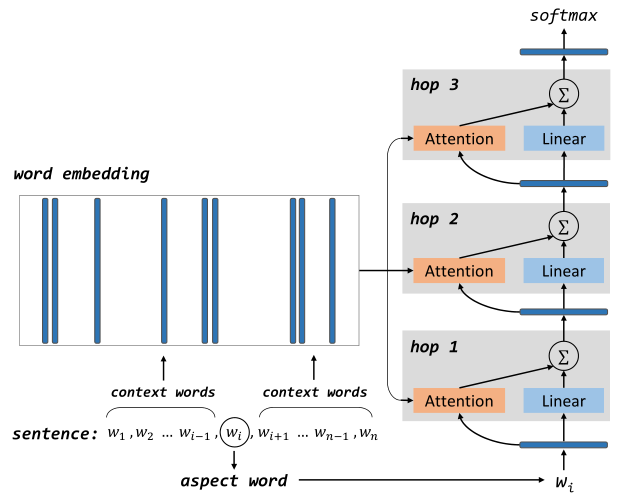
\includegraphics[width=0.7\textwidth]{tang_memory_network.png}
	\caption{The deep memory network approach for targeted sentiment analysis, with 3 hops. The model stored the context of a target in memory and repeatedly attends to that memory with respect to the target word $w_i$. \cite{tang2016}}
	\label{fig:tang_memory_network}
\end{figure}

\subsection{What are some targeted sentiment analysis approaches that use memory networks?}
Memory networks were first put forward towards the goal of targeted sentiment analysis by \cite{tang2016} (figure \ref{fig:tang_memory_network}). Their approach was inspired by \cite{sukhbaatar2015}, with some differences in the attention function that was used, opting instead to use the method put forward in \cite{bahdanau2014}. The authors reported results outperforming the state-of-the-art SVM-based model by \cite{kiritchenko}, which required extensive manual feature engineering, absent from their proposed memory network, as well as the far more complex LSTM based models \cite{tang2016} which required substantially more time to train. Similar to \cite{sukhbaatar2015}, the authors noted a marginal increase in performance as they increased the number of computational hops, which capped at around 8 hops.

\cite{chen2017} construct a location-weighted memory module from the hidden states of a BLSTM placed between the input and the attention modules so as to better capture information from phrases comprising of multiple words, such as \enquote{not wonderful enough}. Moreover, unlike the \cite{tang2016}, they combine the results of their recurrent attention layers non-linearly. These improvements led to a performance boost over \cite{tang2016}. The proposed model architecture is illustrated in figure \ref{fig:chen_recurrent_attention_model}. It is also worth pointing out that the authors failed to reproduce the results originally cited in \cite{tang2016}.

\begin{figure}[!ht]
	\centering
	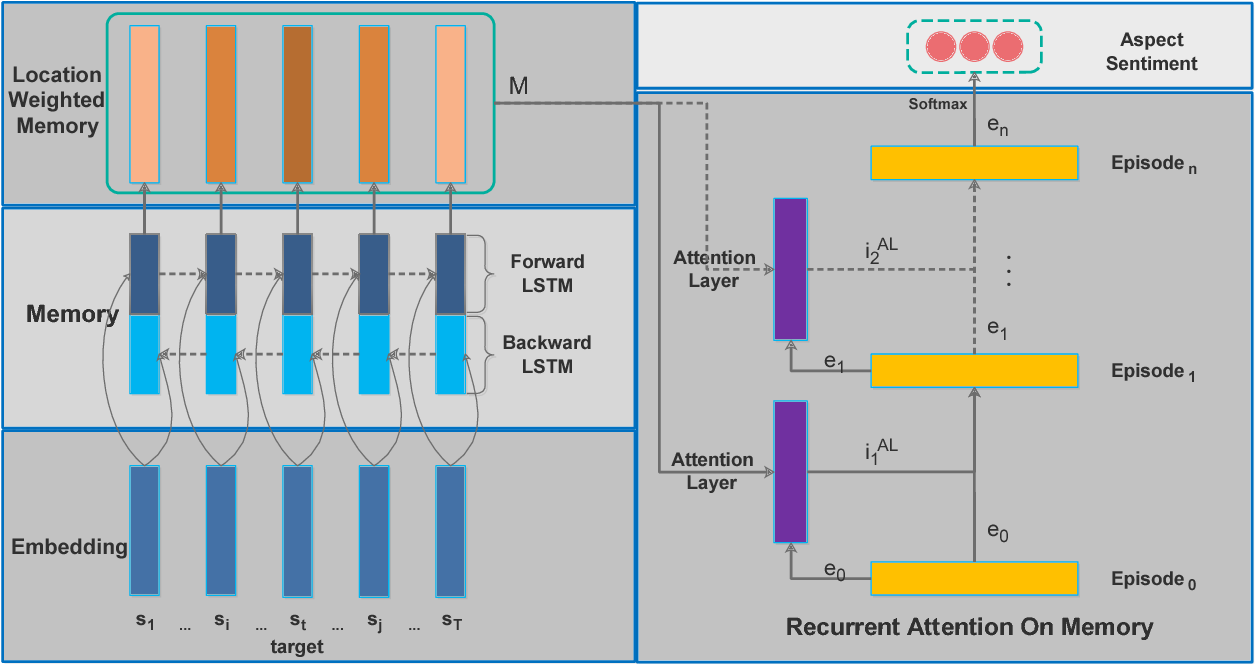
\includegraphics[width=0.7\textwidth]{chen_recurrent_attention.png}
	\caption{The recurrent attention model architecture showing the placement of the location-weighted memory module with respect to the input and attention layers. As opposed to \cite{tang2016}, the attention values are combined from one episode to the next non-linearly, using a GRU. \cite{chen2017}}
	\label{fig:chen_recurrent_attention_model}
\end{figure}

\cite{liu2018} maintain a memory chain of entities that are encountered while processing a phrase and develop a gating mechanism that determines how those memory chains should be updated. The gating mechanism accounts for the content and the location of the memory chains compared to the current input, as well as the past activations, through the use of a GRU unit, when choosing to update a particular memory element.

\subsection{Why is it imperative to attend to targets as well as contexts?}
Recently, work carried out by \cite{wang2018} showed an interesting performance boundary on approaches to targeted sentiment analysis that make use of attention mechanisms. In particular, \cite{wang2018} note that when context words have diametrically opposing sentimental bearings based on the target being considered, this cannot be modelled by improving by attending to the context alone.

To illustrate this, \cite{wang2018} consider two different targets, \textit{price} and \textit{resolution}, in four different phrases; \enquote{high price}, \enquote{low resolution}, \enquote{high resolution} and, \enquote{high price}. Some sentiment score, $s$, for these phrases, where $s < 0$ implies a negative sentiment and $s > 0$ implies a positive sentiment accordingly (eq. \ref{eq:sentiment_score}). The attention weight $\alpha$ will have a value of 1 since the context consists of a single word which is represented by $h$. $v$ represents the target and $W$ is the weight matrix the model must learn.

\begin{equation} \label{eq:sentiment_score}
	s = W(\sum_{i=1}^{n}\alpha_{i}h_{i}+v) = W(h+v)
\end{equation}

From equation \ref{eq:sentiment_score}, the following inequalities can be obtained,
\begin{equation*}
	\begin{split}
		W(h_{high}+v_{price}) < 0 \\
		W(h_{low}+v_{price}) > 0 \\
		W(h_{high}+v_{resolution}) > 0 \\
		W(h_{low}+v_{resolution}) < 0
	\end{split}
\end{equation*}
Expanding these inequalities results in $Wh_{high}<Wh_{low}<Wh_{high}$, which is a contradiction, and can therefore not be learned by the model. \cite{wang2018} point out that this condition cannot be rectified through further attending to the context but rather ameliorating the representation of the targets $v$ to better capture the complex relationship they have with the context in a way that possibly reverses the polarity of the final sentiment score $s$.

Towards this end, \cite{wang2018} experiment using a series of techniques, and note an improvement over previously cited results as well as a direct improvement on the RAM model \cite{chen2017} when these are coupled with their optimally performing target-sensitive context modelling strategy.
\end{document}